\documentclass[12pt,norsk,a4paper]{article}
\usepackage[norsk]{babel}
\usepackage[norsk]{isodate}
\usepackage[T1]{fontenc}
\usepackage{parskip}
\usepackage{url}
\usepackage{cancel}
\usepackage{mathtools}
\usepackage{xfrac}
\usepackage{listings}
\author{Frida Berge (fridatbe)}
\title{IN3140 --- Obligatorisk oppgave 3}
\date{\today}
\usepackage[small,euler-digits]{eulervm}
\usepackage{color}
% \usepackage{minted}
\usepackage{xcolor}
\definecolor{LightGray}{gray}{0.9}
\usepackage{a4wide}
\usepackage[top=2cm]{geometry}
\usepackage{graphicx}
\graphicspath{ {./fig/} }
\newcommand{\tuple}[1]{\ensuremath{\langle #1\rangle}}
\newcommand{\set}[1]{\ensuremath{\{#1\}}}
\newcommand{\imp}{\ensuremath{\rightarrow}}
\newcommand{\M}{\ensuremath{\mathcal{M}}}
\newcommand{\AF}{edge from parent[draw=none]}
\newcommand{\NODE}[1]{\{node \{\ensuremath{#1}\}\}}
\usepackage[explicit]{titlesec}
\titleformat{\section}{\normalfont\Large\bfseries}{}{0em}{#1\ \thesection}


\begin{document}
    \maketitle
    \renewcommand{\thesubsection}{(\alph{subsection})}
    \newpage
    \section{Task}
    \textbf{1a)}\\
    Because the particle moves in a vertical movement it is parallell to the z-axsis. 
    So we have the height $h = y$. 
    If we derivate the point we have the velocity $v = y' = \dot y$.
    And if we derivate the velocity we have the acceleration $a = v' = y'' = \ddot y$
    We know that the langrangian for the particle is the potential energy minus the kinetic energy $(\mathcal{L} = K - P)$.\\
    The formula for the potential therefore is:
    \[P = mgh = mgy\]
    And the formula for the kinetic energy is:
    \[K = \frac{1}{2}mv^2 = \frac{1}{2}m\dot y^2\]
    And if we put it toghether:\\
    \[L = K-P = \frac{1}{2}m\dot y^2 - mgy\]
    From here to find the force (f) we must derivate L with respect to the time derivated to $\dot q$ which in this case equals $\dot y$ (like with a prismatic joint).
    And subtract the derivative of the langrangian with respect to $q$ which in this case is $y$.
    So we have:
    \[\frac{\partial L}{\partial \dot q} = \frac{\partial L}{\partial \dot y} = m\dot y\]
    \[\frac{d}{dt}\frac{\partial L}{\partial \dot q} = \frac{d}{dt}\frac{\partial L}{\partial \dot y} = m\ddot y\]
    \[\frac{\partial L}{\partial q} = \frac{\partial L}{\partial y} = -mg\]
    \[f = \frac{d}{dt}\frac{\partial L}{\partial \dot q} - \frac{\partial L}{\partial q} = \frac{d}{dt}\frac{\partial L}{\partial \dot y} - \frac{\partial L}{\partial y} = m\ddot y+mg\]
    And if we rearrange the equation we get:

    \[\underline{m\ddot y = f - mg}\]
    \newpage


    \textbf{1b)}\\
    % Derive the Lagrangian

    From equation 9 in the task we have:\\
    \[J = \underline{\left[\begin{array}{ccc}
        -s_1(L_2c_2+L_3c_{23}) & -c_1(L_2s_2+L_3s_{23}) & -c_1(L_3s_{23})\\
        c_1(L_2c_2+L_3c_{23}) & -s_1(L_2s_2+L_3s_{23}) & -s_1(L_3s_{23})\\
        0 & L_2c_2+L_3c_{23} & L_3c_{23}\\
        0 & s_1 & s_1\\
        0 & -c_1 & -c_1\\
        1 & 0 & 0
    \end{array}\right]} \]

    Finding the potential energy:\\
    \[P = P_1 + P_2 = m_1gh_1 + m_2gh_2\]
    \begin{itemize}
        \item Because the first mass is evenly distributed, the mass center is found in the middle of link 1, 
                so the height from the base of the robot to $m_1$ is half the length of link 1.
        \item Because the second mass is a point mass located at joint 3 (end of link 2), 
                the height from the base of the robot to $m_2$ is defined as the z-coordonate in the matrix $T_2^0$
                which is $L_1+L_2s_2$ (the sign for $L_2s_2$ is changed from my first assignment because the configuration in this task is flipped 180 degrees from my configuration)
    \end{itemize}
    So the total potential energy is:
    \[P = m_19.81\frac{1}{2}L_1 + m_29.81(L_1+L_2s_2)\]
    \[= \underline{m_19.81\frac{1}{2}L_1+m_2L_19.81+m_2L_2s_29.81}\]

    Finding the kinetic energy:\\
    \[K = K_1+K_2 = \frac{1}{2}m_1v_1^Tv_1 + \frac{1}{2}\omega_1^TI_1\omega_1 + \frac{1}{2}m_2v_2^Tv_2 + \frac{1}{2}\omega_2^TI_2\omega_2\]
    
    Starting with the linear potential energy (uses the 1. and 2. column of the jacobian in the assignment because we only use two links in this task):\\
    \[v_1 = J_{v_1}\dot q = 
    \left[\begin{array}{cc}
        -s_1(L_2c_2+L_3c_{23}) & -c_1(L_2s_2+L_3s_{23})\\
        c_1(L_2c_2+L_3c_{23}) & -s_1(L_2s_2+L_3s_{23})\\
        0 & L_2c_2+L_3c_{23}\\
    \end{array}\right]
    \left[\begin{array}{c}
        \dot\theta_1 \\ \dot\theta_2
    \end{array}\right]\]
    Sets all values related to $\theta_2$ and $\theta_3$ to 0:\\
    \[=\left[\begin{array}{cc}
        0 & 0\\
        0 & 0\\
        0 & 0\\
    \end{array}\right]
    \left[\begin{array}{c}
        \dot\theta_1 \\ \dot\theta_2
    \end{array}\right]
    = \left[\begin{array}{c}
        0 \\ 0 \\ 0
    \end{array}\right]\]

    \[v_2 = J_{v_2}q = 
    \left[\begin{array}{cc}
        -s_1(L_2c_2+L_3c_{23}) & -c_1(L_2s_2+L_3s_{23})\\
        c_1(L_2c_2+L_3c_{23}) & -s_1(L_2s_2+L_3s_{23})\\
        0 & L_2c_2+L_3c_{23}\\
    \end{array}\right]
    \left[\begin{array}{c}
        \dot\theta_1 \\ \dot\theta_2
    \end{array}\right]\]

    Sets all values related to $\theta_3$ to 0:\\
    \[= \left[\begin{array}{cc}
        -s_1(L_2c_2) & -c_1(L_2s_2)\\
        c_1(L_2c_2) & -s_1(L_2s_2)\\
        0 & L_2c_2\\
    \end{array}\right]
    \left[\begin{array}{c}
        \dot\theta_1 \\ \dot\theta_2
    \end{array}\right]
    = \left[\begin{array}{c}
        -\dot\theta_1s_1(L_2c_2)-\dot\theta_2c_1(L_2s_2)\\
        \dot\theta_1c_1(L_2c_2)-\dot\theta_2s_1(L_2s_2)\\
        \dot\theta_2L_2c_2\\
    \end{array}\right]\]

    Calculating $v_1^2$ and $v_2^2$:
    \[v_1^2 = 0\]
    \[v_2^2 = v_2^Tv_2\]
    \[=\left[\begin{array}{ccc}
        -\dot\theta_1s_1L_2c_2-\dot\theta_2c_1L_2s_2&
        \dot\theta_1c_1L_2c_2-\dot\theta_2s_1L_2s_2&
        \dot\theta_2L_2c_2\\
    \end{array}\right]
    \left[\begin{array}{c}
        -\dot\theta_1s_1L_2c_2-\dot\theta_2c_1L_2s_2\\
        \dot\theta_1c_1L_2c_2-\dot\theta_2s_1L_2s_2\\
        \dot\theta_2L_2c_2\\
    \end{array}\right]\]
    \[= (-\dot\theta_1s_1L_2c_2)^2+ \cancel{2\dot\theta_1s_1L_2c_2\dot\theta_2c_1L_2s_2} + (-\dot\theta_2c_1L_2s_2)^2\]
    \[+ (\dot\theta_1c_1L_2c_2)^2 - \cancel{2\dot\theta_1c_1L_2c_2\dot\theta_2s_1L_2s_2} + (-\dot\theta_2s_1L_2s_2)^2\]
    \[+ (\dot\theta_2L_2c_2)^2\]
    \vspace{3mm}
    \[= (\dot\theta_1s_1L_2c_2)^2 + (\dot\theta_1c_1L_2c_2)^2 + (\dot\theta_2c_1L_2s_2)^2 + (\dot\theta_2s_1L_2s_2)^2 + (\dot\theta_2L_2c_2)^2\]
    \[= \cancel{(s_1^2+c_1^2)}(\dot\theta_1L_2c_2)^2 + \cancel{(s_1^2+c_1^2)}(\dot\theta_2L_2s_2)^2 + (\dot\theta_2L_2c_2)^2\]
    \[= (\dot\theta_1L_2c_2)^2 + (\dot\theta_2L_2s_2)^2 + (\dot\theta_2L_2c_2)^2\]
    \[= (\dot\theta_1L_2c_2)^2 + \cancel{(s_2^2+c_2^2)}(\dot\theta_2L_2)^2\]
    \[= \underline{\dot\theta_1^2L_2^2c_2^2 + \dot\theta_2^2L_2^2}\]


    Then calculates the angular potential energy:\\

    \[\omega_1 = J_{\omega_1}\dot q = 
    \left[\begin{array}{cc}
        0 & s_1\\
        0 & -c_1\\
        1 & 0\\
    \end{array}\right]
    \left[\begin{array}{c}
        \dot\theta_1 \\ \dot\theta_2
    \end{array}\right]\]
    
    Sets the second coulmn to 0:\\
    \[\omega_1 = J_{\omega_1}\dot q = 
    \left[\begin{array}{cc}
        0 & 0\\
        0 & 0\\
        1 & 0\\
    \end{array}\right]
    \left[\begin{array}{c}
        \dot\theta_1 \\ \dot\theta_2
    \end{array}\right]
    = \left[\begin{array}{c}
        0\\
        0\\
        \dot\theta_1\\
    \end{array}\right]\]

    \[\omega_2 = J_{\omega_2}\dot q = 
    \left[\begin{array}{cc}
        0 & s_1\\
        0 & -c_1\\
        1 & 0\\
    \end{array}\right]
    \left[\begin{array}{c}
        \dot\theta_1 \\ \dot\theta_2
    \end{array}\right]
    = \left[\begin{array}{c}
        \dot\theta_2s_1\\
        -\dot\theta_2c_1\\
        \dot\theta_1\\
    \end{array}\right]\]

    Calculating the Inertia from inertia tensors:\\
    \[I_1 = \left[\begin{array}{ccc}
        0 & 0 & 0\\
        0 & 0 & 0\\
        0 & 0 & \frac{m_1r_1^2}{2}
    \end{array}\right] \hspace{10mm} I_2 = \left[\begin{array}{ccc}
        0 & 0 & 0\\
        0 & 0 & 0\\
        0 & 0 & 0
    \end{array}\right]\]

    \[\mathcal{I}_1 = R_{z,\theta1}I_1R_{z,\theta1}^T 
    = \left[\begin{array}{ccc}
        c_1 & -s_1 & 0\\
        s_1 & c_1 & 0\\
        0 & 0 & 1
    \end{array}\right]\left[\begin{array}{ccc}
        0 & 0 & 0\\
        0 & 0 & 0\\
        0 & 0 & \frac{m_1r_1^2}{2}
    \end{array}\right]\left[\begin{array}{ccc}
        c_1 & s_1 & 0\\
        -s_1 & c_1 & 0\\
        0 & 0 & 1
    \end{array}\right]
    = \left[\begin{array}{ccc}
        0 & 0 & 0\\
        0 & 0 & 0\\
        0 & 0 & \frac{m_1r_1^2}{2}
    \end{array}\right]\]

    \[\mathcal{I}_2 = R_{x,\theta_2}I_2R_{x,\theta2}^T 
    = \left[\begin{array}{ccc}
        1 & 0 & 0\\
        0 & c_2 & -s_2\\
        0 & s_1 & c_2
    \end{array}\right]\left[\begin{array}{ccc}
        0 & 0 & 0\\
        0 & 0 & 0\\
        0 & 0 & 0
    \end{array}\right]\left[\begin{array}{ccc}
        1 & 0 & 0\\
        0 & c_2 & s_2\\
        0 & -s_2 & c_2
    \end{array}\right]
    = \left[\begin{array}{ccc}
        0 & 0 & 0\\
        0 & 0 & 0\\
        0 & 0 & 0
    \end{array}\right]\]

    Total kinetic energy:\\
    \[K = K_1+K_2\]
    \[K_1 = \frac{1}{2}m_1v_1^Tv_1 + \frac{1}{2}\omega_1^T\mathcal{I}_1\omega_1\]
    \[\frac{1}{2}m_1*0 + \frac{1}{2}
                                            \left[\begin{array}{ccc}0&0&\dot\theta_1\end{array}\right]
                                            \left[\begin{array}{ccc}0&0&0\\0&0&0\\0&0&\frac{m_1r_1^2}{2}\end{array}\right]
                                            \left[\begin{array}{c}0\\0\\\dot\theta_1\end{array}\right]\]
    \[= \frac{1}{2}
                    \left[\begin{array}{ccc}0&0&\dot\theta_1\end{array}\right]
                    \left[\begin{array}{c}0\\0\\\dot\theta_1\frac{m_1r_1^2}{2}\end{array}\right]
    = \frac{1}{2}\dot\theta_1^2\frac{m_1r_1^2}{2} = \underline{\frac{m_1\dot\theta_1^2r_1^2}{4}}\]
    \vspace{5mm}
    \[K_2 = \frac{1}{2}m_2v_2^Tv_2 + \frac{1}{2}\omega_2^T\mathcal{I}_2\omega_2\]
    \[= \frac{1}{2}m_2(\dot\theta_1^2L_2^2c_2^2+\dot\theta_2^2L_2^2) + \frac{1}{2}
                                                                    \left[\begin{array}{ccc}\dot\theta_2s_1&-\dot\theta_2c_1&\dot\theta_1\end{array}\right]
                                                                    \left[\begin{array}{ccc}0&0&0\\0&0&0\\0&0&0\end{array}\right]
                                                                    \left[\begin{array}{c}\dot\theta_2s_1\\-\dot\theta_2c_1\\\dot\theta_1\end{array}\right]\]
    \[= \frac{1}{2}m_2(\dot\theta_1^2L_2^2c_2^2+\dot\theta_2^2L_2^2) + \frac{1}{2}*0 = \underline{\frac{m_2\dot\theta_1^2L_2^2c_2^2+m_2\dot\theta_2^2L_2^2}{2}}\]
  \vspace{5mm}
    \[K = \frac{m_1\dot\theta_1^2r_1^2}{4} + \frac{m_2\dot\theta_1^2L_2^2c_2^2+m_2\dot\theta_2^2L_2^2}{2}\]


    Now we have every part of the equation and can compute the Langrange:\\
    \[\mathcal{L} = K-P = (K_1+K_2)-(P_1+P_2)\]
    \[=(\frac{m_1\dot\theta_1^2r_1^2}{4} + \frac{m_2\dot\theta_1^2L_2^2c_2^2+m_2\dot\theta_2^2L_2^2}{2})-(m_19.81\frac{1}{2}L_1+m_2L_19.81+m_2L_2s_29.81)\]
    \[\mathcal{L} = \underline{\frac{m_1\dot\theta_1^2r_1^2}{4} + \frac{m_2\dot\theta_1^2L_2^2c_2^2}{2}+\frac{m_2\dot\theta_2^2L_2^2}{2}-m_19.81\frac{1}{2}L_1-m_2L_19.81-m_2L_2s_29.81}\]
    \newpage








    
    \textbf{1c)}

    \[\tau_i = \frac{d}{dt}\left(\frac{\partial\mathcal{L}}{\partial\dot q_i}\right)-\frac{\partial\mathcal{L}}{\partial q_i}\]
    Because both joints are revoloute:\\
    \[\tau_i = \frac{d}{dt}\left(\frac{\partial\mathcal{L}}{\partial\dot \theta_i}\right)-\frac{\partial\mathcal{L}}{\partial\theta_i}\]
    
    Starts by calculating $\tau_1$:\\
    \[\frac{\partial\mathcal{L}}{\partial\dot \theta_1} = 
    \frac{m_1\dot\theta_1r_1^2}{2}+m_2\dot\theta_1L_2^2c_2^2\]
    \[\frac{d}{dt}\left(\frac{\partial\mathcal{L}}{\partial\dot\theta_1}\right)= \frac{m_1r_1^2\ddot\theta_1}{2} + m_2L_2^2c_2^2\ddot\theta_1 - 2m_2L_2^2\dot\theta_1\dot\theta_2c_2s_2\]
    \[\frac{\partial\mathcal{L}}{\partial \theta_1} = 0\]
    \[\tau_1 =\frac{m_1r_1^2\ddot\theta_1}{2} + m_2L_2^2c_2^2\ddot\theta_1 - 2m_2L_2^2\dot\theta_1\dot\theta_2c_2s_2\]

    Calculates $\tau_2$:\\
    \[\frac{\partial\mathcal{L}}{\partial\dot \theta_2} = m_2\dot\theta_2L_2^2\]
    \[\frac{d}{dt}\left(\frac{\partial\mathcal{L}}{\partial\dot\theta_2}\right)= m_2 \ddot\theta_2 L_2^2\]
    \[\frac{\partial\mathcal{L}}{\partial \theta_2} = -m_2\dot \theta_1^2L_2^2c_2s_2-m_2L_2c_29.81\]
    \[\tau_2 =  m_2 \ddot\theta_2 L_2^2 + m_2\dot \theta_1^2L_2^2c_2s_2 + m_2L_2c_29.81\]
    
    The Euler-Langrange:\\
    \[\tau = \left[\begin{array}{c} \tau_1 \\ \tau_2\end{array}\right]
    = \left[\begin{array}{c}
        \frac{m_1r_1^2\ddot\theta_1}{2} + m_2L_2^2c_2^2\ddot\theta_1 - 2m_2L_2^2\dot\theta_1\dot\theta_2c_2s_2\\
        m_2 \ddot\theta_2 L_2^2 + m_2\dot \theta_1^2L_2^2c_2s_2 + m_2L_2c_29.81
    \end{array}\right]\]

    Rewriting to the form $D(q)\ddot q + C(q, \dot q)\dot q + g(q) = \tau$:\\
    \[\tau =\underline{\left[\begin{array}{cc}
                \frac{m_1r_1^2}{2}+m_2L_2^2c_2^2 & 0\\
                0 & m_2L_2^2\\
            \end{array}\right]
            \left[\begin{array}{c}
                \ddot \theta_1\\
                \ddot \theta_2\\
            \end{array}\right]
            +\left[\begin{array}{cc}
                -m_2L_2^2c_2s_2\dot\theta_2 & -m_2L_2^2c_2s_2\dot\theta_1\\
                m_2L_2^2c_2s_2\dot\theta_1 & 0\\
            \end{array}\right]
            \left[\begin{array}{c}
                \dot \theta_1\\
                \dot \theta_2\\
            \end{array}\right]
            +\left[\begin{array}{c}
                0\\
                m_2L_2c_29.81\\
            \end{array}\right]}\]

    \newpage





    \section{Task}
    \textbf{2a)}\\
    Because the potential energy is defined by $\sum_{i=1}^{n}m_ig^Tr_{ci}$ where n = 3 (because we have three links)
    the total potential energy can be found by using this expression to calculate the potential energy in each of the three
    masses and add them together. The mass is defined in the task, and so is g. I found $r_{ci}$ by making a 
    list of matrixes (r1, r2 and r3) which are the z-coordinates (the last column/translation) of the three matrixes $H_1^0$, $H_2^0$ and $H_3^0$
    found from assignment 1 and 2. In each of the links the mass is located in the middle of the link. Therefore in link 1, I divided the height by 2,
    in link 2 i divided all variables related to link 2 by 2, and the same for link 3. This represents the height of the mass because the z-coordinate 
    of the baseframe of the robot (coordinatesystem $x_0y_0z_0$) points straight upswards, and becomes the height related to the base.\\\\
    Code:
    \begin{lstlisting}
    def pot():
        prod1 = mass[0]*g.T*r[0]
        prod2 = mass[1]*g.T*r[1]
        prod3 = mass[2]*g.T*r[2]
        return prod1+prod2+prod3
    
    def main():
        print("Potential energy:")
        pretty_print(pot())
    \end{lstlisting}
    Output:\\
    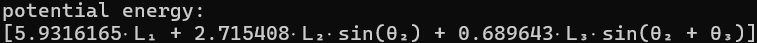
\includegraphics[width=\textwidth]{pot.png}\\

    







    \newpage
    \textbf{2b)}\\
    To calculate the kinetic energy i used the formula in the assignment\\
    $\frac{1}{2}\dot q^T\left[\sum_{i=1}^{n}m_iJ_{vi}(q)^TJ_{vi}(q)+J_{wi}(q)^TR_i(q)I_iR_i(q)^TJ_{wi}(q)\right]\dot q$
    Where n = 3 because there are three masses. The masses are given in the assignment, where $m_i$ represent the mass of mass point i.
    $J_{vi}(q)$ represents the first three rows in the jacobian, and $J_{wi}(q)$ represents the last three rows of the jacobian.
    The R matrix is the rotational matrix for each mass related to the baseframe, where the first matrix was given in the task, 
    and the others where calculated by matrix multiplication with a z-rotation matrix.
    To calculate each joint by it self I matrix multiplied with a diagonal matrix so that the other non-relevant columns was set to zero,
    and to changed all non-relevant values to zero by using the function 'subs'. 
    To calculate the total kinetic energy i added the kinetic   energy from each mass.\\\\
    
    Code:
    \begin{lstlisting}
    def kin():
        col1 = diag(1,0,0)
        col2 = diag(1,1,0)
        Jv1 = Jv.subs([(cos(theta2), 0),
                       (cos(theta3), 0),
                       (sin(theta2), 0),
                       (sin(theta3), 0),
                       (cos(theta2+theta3), 0),
                       (sin(theta2+theta3), 0),
                       (L2, 0),  
                       (L3, 0)])
        Jv2 = Jv.subs([(cos(theta3), 0),
                        (sin(theta3), 0),
                        (cos(theta2+theta3), 0),
                        (sin(theta2+theta3), 0),
                        (L3, 0)])
        Jv3 = Jv
        Jw1 = Jw.subs([(cos(theta2), 0), 
                       (cos(theta3), 0), 
                       (sin(theta2), 0),  
                       (sin(theta3), 0), 
                       (cos(theta2+theta3), 0),
                       (sin(theta2+theta3), 0),
                       (L2, 0),  (L3, 0)])
        Jw2 = Jw.subs([(cos(theta3), 0),
                       (sin(theta3), 0),
                       (cos(theta2+theta3), 0),
                       (sin(theta2+theta3), 0),
                       (L3, 0)])
        Jw3 = Jw

        k1v = mass[0]*(Jv1*col1).T*Jv1*col1
        k1w = (Jw1*col1).T*M1*I1*M1.T*Jw1*col1
        k1 = k1v+k1w

        k2v = mass[1]*Jv2*col2.T*Jv2*col2
        k2w = (Jw2*col2).T*M2*I2*M2.T*Jw2*col2
        k2 = k2v+k2w

        k3v = mass[2]*Jv3*Jv3
        k3w = Jw3.T*M1*I1*M3.T*Jw3
        k3 = k3v+k3w

        return k1+k2+k3

    def main():
        print("Kinetic energy:")
        D = kin()
        K = (1/2)*qdot.T*(D)*qdot
        pretty_print(K)
    \end{lstlisting}
    Output:\\
    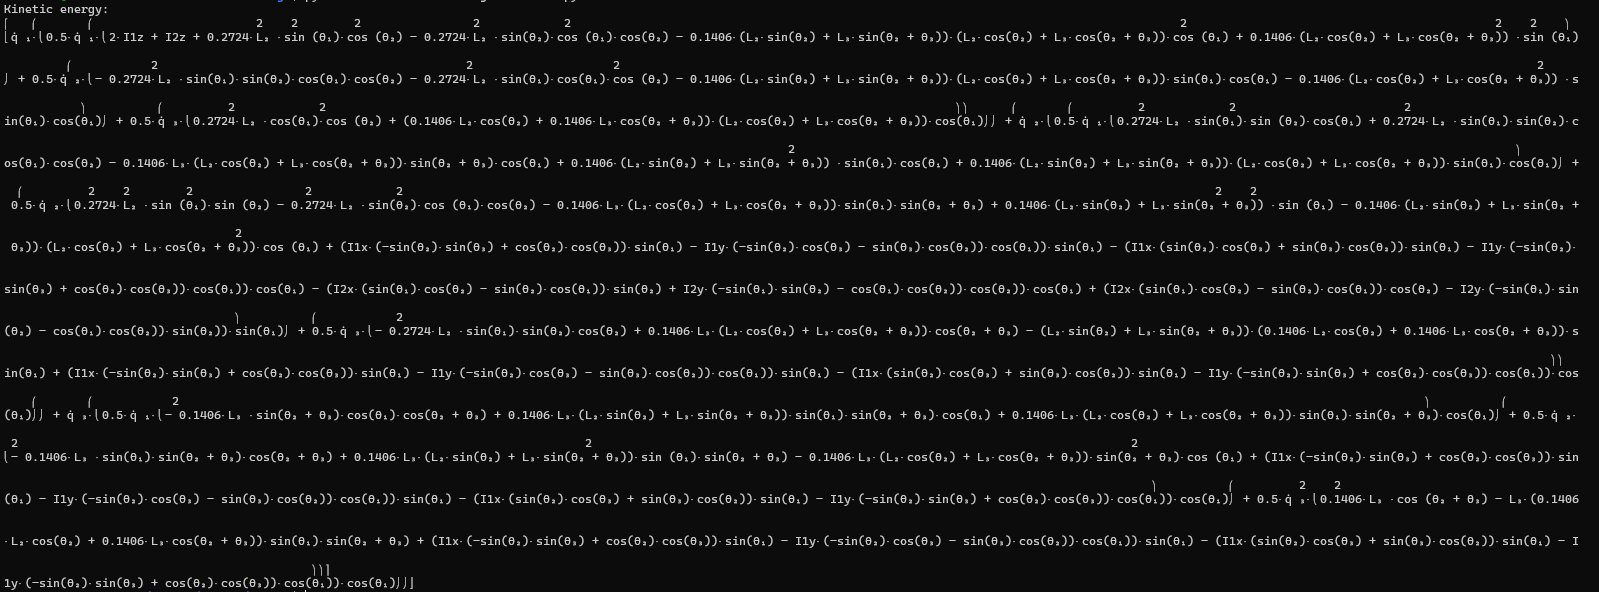
\includegraphics[width=\textwidth]{ouput.png}\\









    \newpage
    \textbf{2c)}\\
    % se side 183 i boka
    \[\tau = D(q)\ddot q + C(q,\dot q)\dot q +g(q)\]
    Can be written as:
    \[\left[\begin{array}{c} \tau_1 \\ \tau_2 \\ \tau_3 \end{array}\right] = \]
            \[\left[\begin{array}{ccc}
                    d_{11}(q) & d_{12}(q) & d_{13}(q)\\
                    d_{21}(q) & d_{22}(q) & d_{23}(q)\\
                    d_{31}(q) & d_{32}(q) & d_{33}(q)
                \end{array}\right] \left[\begin{array}{c} \ddot q1 \\ \ddot q2 \\ \ddot q3 \end{array}\right]
            +\left[\begin{array}{ccc}
                c_{11}(q,\dot q) & c_{12}(q,\dot q) & c_{13}(q,\dot q)\\
                c_{21}(q,\dot q) & c_{22}(q,\dot q) & c_{23}(q,\dot q)\\
                c_{31}(q,\dot q) & c_{32}(q,\dot q) & c_{33}(q,\dot q)
            \end{array}\right] \left[\begin{array}{c} \dot q_1 \\ \dot q_2 \\ \dot q_3 \end{array}\right]
            +\left[\begin{array}{c}
                g_1(q) \\ g_2(q) \\ g_3(q)
            \end{array}\right]\]

    Where $d_{ij}$ are elements of matrix D, $c_{ij}$ are elements of matrix C, $g_k$ are elements of matrix g, $\tau_k$ are elements of matrix $\tau$, $\ddot q_k$ are elements of matix $\ddot q$ and $\dot q$ are elements of matix $\dot q$

    \[\left[\begin{array}{c} \tau_1 \\ \tau_2 \\ \tau_3 \end{array}\right] = \]
            \[\left[\begin{array}{c}
                    d_{11}(q)\ddot q_1 + d_{12}(q)\ddot q_2 + d_{13}(q)\ddot q_3\\
                    d_{21}(q)\ddot q_1 + d_{22}(q)\ddot q_2 + d_{13}(q)\ddot q_3\\
                    d_{31}(q)\ddot q_1 + d_{32}(q)\ddot q_2 + d_{33}(q)\ddot q_3
                \end{array}\right]
            +\left[\begin{array}{c}
                c_{11}(q,\dot q)\dot q_1 + c_{12}(q,\dot q)\dot q_2 + c_{13}(q,\dot q)\dot q_3\\
                c_{21}(q,\dot q)\dot q_1 + c_{22}(q,\dot q)\dot q_2 + c_{23}(q,\dot q)\dot q_3\\
                c_{31}(q,\dot q)\dot q_1 + c_{32}(q,\dot q)\dot q_2 + c_{33}(q,\dot q)\dot q_3
            \end{array}\right]
            +\left[\begin{array}{c}
                g_1(q) \\ g_2(q) \\ g_3(q)
            \end{array}\right]\]

    And if you only view one row which represents one mass (k):
    \[\tau_k = (d_{k1}(q)\ddot q_1 + d_{k2}(q)\ddot q_2 + d_{k3}(q)\ddot q_3) + (c_{k1}(q,\dot q)\dot q_1 + c_{k2}(q,\dot q)\dot q_2 + c_{k3}(q,\dot q)\dot q_3) + (g_k(q))\]

    Then we can put up some summations for the $\ddot q_j$ and $\dot q_j$, where n would be 3 in our case because we have 3 masses\\
    \[\tau_k = \sum_{j=i}^{3}(d_{kj}(q)\ddot q_j) + \sum_{j = 1}^{3}(c_{kj}(q,\dot q)\dot q_j) + (g_k(q))\]
    Where j is the index of each column in D and C. And from the texbook (page 183) we have that:
    \[c_{kj} = \sum_{i=1}^{n}c_{ij}(q)\dot q_i\]
    So we can write the expression like this:
    \[\tau_k = \underline{\sum_{j=i}^{3}(d_{kj}(q)\ddot q_j) + \sum_{i = 1}^{3}\sum_{j = 1}^{3}(c_{ij}(q)\dot q_i\dot q_j) + (g_k(q))}\]



    Forces reprecented by\dots
        \begin{itemize}
            \item $D(q)$ - the inertia (nxn), and multiplied with $\ddot q$ expresses the acceleration for the motion (nx1)
            \item $C(q,\dot q)$ - the coriolis (nxn) (centrifugal forces), and multiplied with $\dot q$ expresses the quadric velocity (nx1)
            \item $g(q)$ - the gravitational force (nx1)
        \end{itemize}





    \newpage
    \textbf{2d)}\\
    % d) 20 Compute the two remaining terms of equation
    % C(q) og g(q)
    The two remaining expressions are for $C(q,\dot q)$:
    \[c_{kj} = \sum_{i=1}^{n}c_{ij}(q)\dot q_i = \sum_{i=1}^{n}\frac{1}{2}\left(\frac{\partial d_{kj}}{\partial q_1}+\frac{\partial d_{ki}}{\partial q_j}-\frac{\partial d_{ij}}{\partial q_k}\right)\dot q_i\]
    And the for g(q):
    \[g(q) = (g_1(q), ... , g_n(q))\]
    To calculate the D matrix I filled out the variables in the formula above. And g is given by [0 0 9.81$]^T$\\\\
    Code:
    \begin{lstlisting}
    def cor(D):
        C = zeros(3,3)
        for k in range(3):
            for j in range(3):
                for i in range(3):
                    C[k,j] = (1/2)*(diff(D[k,j],thetas[i])
                            +diff(D[k,i],thetas[j])
                            -diff(D[i,j], thetas[k]))*qdot[i]
        return C
    
    main():
        print("g(q):")
        pretty_print(g)
        print("\nC(q,qdot):")
        C = cor(D)
        pretty_print(C)
    \end{lstlisting}
    Output (only for g because C was way too long):\\
    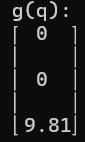
\includegraphics[width=0.1\textwidth]{g.png}\\





    \newpage
    \textbf{2e)}\\
    To assemble each $\tau_i$ I multiplied $D(q)$(3x3) with $\ddot q$(3x1) and $C(q,\dot q)$(3x3) with $\dot q$(3x1).
    And then added all the parts together.\\\\
    Code:
    \begin{lstlisting}
    def tau(D,C,g):
        tau = zeros(3,1)
        Dpart = D*qdotdot
        Cpart = C*qdot
        return Dpart+Cpart+g
    
    def main():
        t = tau(D,C,g)
        pretty_print(t)

    \end{lstlisting}

    % e) 5 Compute the dynamical model (τ ) of the three-link manipulator and
    % submit your code (submitting the output is not necessary).
    % (3x1)
        
\end{document}